The envisioned fourth industrial revolution has set the track for modern advancements in achieving a global web of pervasive connectivity between all sorts of machines \cite{akyildiz2005wireless, cilfone2019wireless}. New means of radio and wireless communication have been pushing for the technological heterogeneity of protocols, architectures, devices, and consequent performance levels, in order to find their design suitability for different coverage or range scenarios, transmission or bandwidth rates \cite{sichitiu2005wireless}. Additionally, requirements for more complex, adaptable, and resilient topologies have captured broad interest, in both academic and industry domains. 

\begin{figure} [ht]
  \begin{center}
  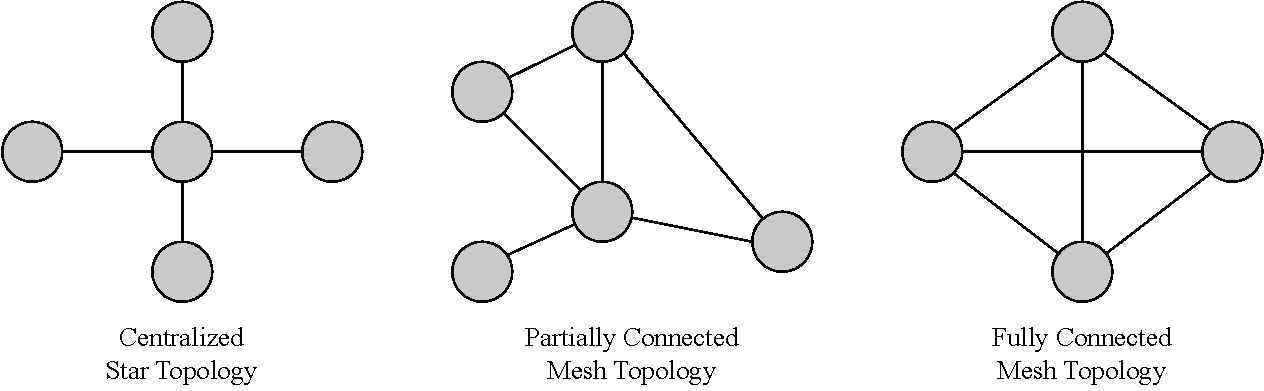
\includegraphics[width=0.9\textwidth]{network-topologies.pdf}
  \caption{Examples of different topologies of a computer network. Starting on the left, the star topology shows all the nodes connected to a central hub. To the right, examples of mesh topologies depict the direct and decentralized connections between the nodes.}
  \label{fig:mesh-network-topology}
  \end{center}
\end{figure}

The development of new hardware, protocols, and applications started gaining momentum and branched their way forward to support the popularisation of Wireless Mesh Networks (WMNs). In mesh topologies (see Figure~\ref{fig:mesh-network-topology}), network nodes are directly and dynamically connected in a non-hierarchical way. This trait eventually allows for many-to-many communications between the devices, to efficiently route data from a generic source to a generic destination. The infrastructure nodes that make up the mesh are expected to dynamically self-organize and configure themselves, resulting in beneficial distributed effects on the overall fault tolerance, ease of deployment, and workload allocation \cite{cilfone2019wireless, sichitiu2005wireless}. WMNs follow these principles with the particularity of being made up of radio nodes that communicate via any sort of wireless technology.

Some of the most common wireless technologies that have been, throughout the years, ported to WMNs are Bluetooth, LoRa and IEEE 802.11. The first two are prominent solutions for the extremities of the mesh networking spectrum, with Bluetooth under the short-range realm of Personal Area Networks (PANs), and LoRa  under the Low Power, Wide Area (LPWA) scenario. Downsides of these technologies are, respectively, the limiting coverage range for one-hop neighborhoods, or the low bandwidth rates \cite{cilfone2019wireless}. Hence, IEEE 802.11 became the most flexible and widely used, being the basis of the Wi-Fi standard, which, at the beginning of the last decade, saw an amendment that mainly targeted mesh networks~\textemdash~the IEEE 802.11s WLAN Mesh Standard \cite{hiertz2010ieee}. The novelty came with the introduction of routing mechanisms operating at the ISO/OSI Layer 2, allowing for compatible information delivery in the layers above. The dynamic establishment of a topology for IEEE 802.11s-based mesh networks relies on the phased transmission of beacon messages that allow for the discovery, synchronization, and maintenance of the links between the peers. IEEE 802.11s has a default routing protocol, the Hybrid Wireless Mesh Protocol (HWMP), which is based on a series of flooding procedures for both proactive and reactive path finding and selection \cite{bari2012performance}. However, this protocol is not strictly enforced by the standard and has been replaced by other more popular solutions. One notable example is the Better Approach To Mobile Ad-hoc Networks (B.A.T.M.A.N.) routing protocol.

This thesis will explore the concept of WMNs and their potential for serving as the infrastructural topology that enables the relatively short-ranged wireless exchange of messages between the participants of a \pol{} protocol. The following sections will present the B.A.T.M.A.N. routing protocol, OpenWrt and other relevant tools that will be later used to implement the \poc{}.

\subsubsection{B.A.T.M.A.N. Routing Protocol}

The Better Approach To Mobile Ad-hoc Networks (B.A.T.M.A.N.)\footnote{\url{http://www.open-mesh.org/}} is a proactive routing protocol for WMNs that operates not at the network layer but at the data link layer, asserting the reliability of radio links using routing metrics and a distance-vector approach \cite{seither2011routing}. Its newer wireless version, \emph{batman-adv}, has gained traction and popularity and eventually made itself available in the Linux kernel.

Route discovery is preemptively replaced with neighbour discovery, and each infrastructural node is instructed to calculate its potential best next-hop, significantly reducing the overhead of requiring each peer to be aware of the whole network topology. Its version V introduced a throughput metric to evaluate the links' quality and routing choices, replacing the version IV packet loss based metric, deemed unsuitable for larger network sizes \cite{seither2011routing}.

\begin{figure} [ht]
  \begin{center}
  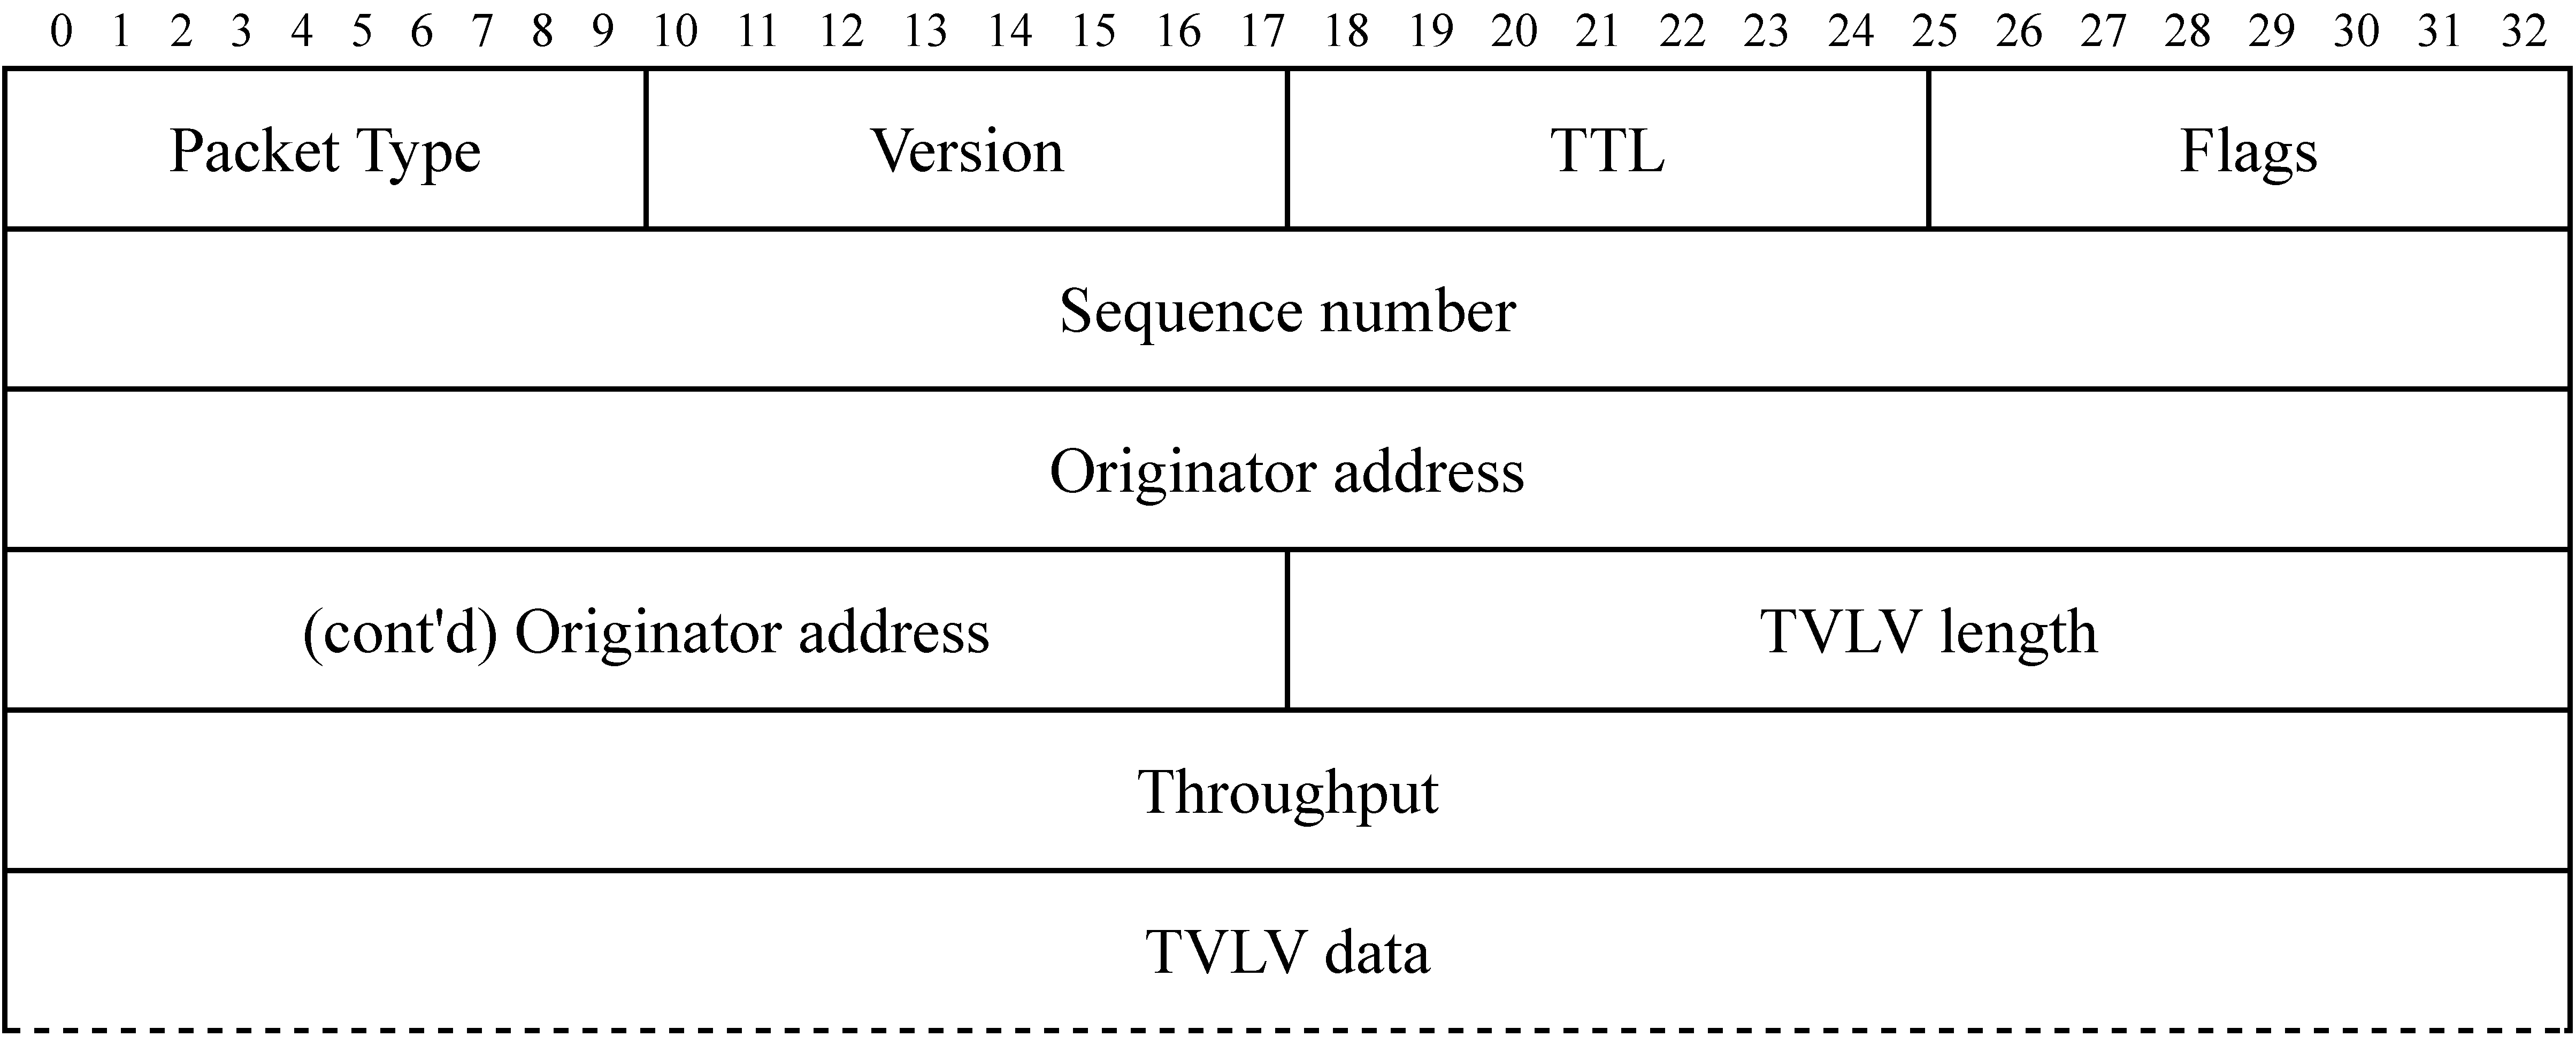
\includegraphics[width=0.9\textwidth]{batman-adv-ogmv2.pdf}
  \caption{OriGinator Message version 2 (OGMv2) packet format \cite{cilfone2019wireless,open-mesh-ogmv2}. These messages are broadcasted with a collision avoidance delay mechanism defaulting to 1 second. The packets contain, among other fields, the originator's MAC address and throughput metric values, measured in units of 100 kbit/s.}
  \label{fig:batman-adv-ogmv2}
  \end{center}
\end{figure}

The discovery of neighbouring nodes is accomplished with the capture of broadcasted OriGinator Messages (OGMv2, see Figure~\ref{fig:batman-adv-ogmv2}), that feature a collision avoidance delay mechanism, the detection of new or duplicate messages, and other fields for throughput measurement and gateway discovery. The Echo Location Protocol (ELP) handles the received messages and ranks the discovered neighbours. The OGM flooding protocol, on the other hand, enables mesh routing procedures that, simultaneously but independently, allow for estimating the quality of the individual links \cite{cilfone2019wireless}. Additionally, the protocol facilitates OGM aggregations as an effort to reduce the overhead of sending many short-sized frames. Nevertheless, there is still a quest for optimizations that would allow for more efficient use of multiple interfaces. An implementation of a subset of the Internet Control Message Protocol (ICMP) is also made available, allowing, for instance, the use of the \emph{ping} command to test the connectivity between nodes \cite{seither2011routing}.

Building on the previous, the B.A.T.M.A.N. routing protocol has been, through multiple initiatives, successfully blended into the OpenWrt project, which will also be employed in the \poc{}. The following section will present OpenWrt and other relatable tools.

\subsubsection{OpenWrt, QEMU, and Raspberry Pis}

The OpenWrt project\footnote{\url{https://openwrt.org/}} is a Linux distribution for embedded devices, which, in the context of this thesis, will serve as the host operating system for running the \poc{} solution. The project is based on the Linux kernel, encapsulating several of its libraries and packages, and is designed to be used on resource-constrained devices. OpenWrt features not only a writable root filesystem and automated build tools with integrated cross-compiler toolchain, but also a package management system that allows for the installation of additional software. The project also provides extensive configuration options for networking capabilities, which includes enabling mesh networking support through the B.A.T.M.A.N. routing protocol. 

To facilitate the development and testing of the \poc{}, the QEMU\footnote{\url{https://www.qemu.org/}} emulator will be used. QEMU is a generic and open-source machine virtualizer that, through its versatile set of features, allows for the full-system emulation of a wide range of hardware and software. The emulator will run the OpenWrt-generated images and spawn multiple virtual machines. These machines will simulate the various protocol participants by establishing, with the help of the network emulation tools, a fully connected mesh network. The intention is to ease and accelerate the development process by allowing for testing the \poc{} in a controlled environment, without the management, maintenance, and deployment hustle of physical devices. Later, the solution is planned to be deployed on a set of Raspberry Pis\footnote{\url{https://www.raspberrypi.org/}}, the most widely used single-board computers for developing IoT solutions. The implementation journey will be documented in Chapter~\ref{sec:proof-of-concept}.
